\chapter{Bolted Connections}\label{ch:bolt}
\section{Connection Types}
Because of experiences in the NZ construction industry, it is common practice not to conduct major structural welding at the construction site. Instead, the preferred method used is `shop welding and site bolting'. This method has advantages in terms of construction speed, simplicity and quality control that are not enjoyed in other countries. However, proper planning is necessary to ensure that the building will fit together properly at the construction site.

Different connections can put different demands on the bolts.
\begin{itemize}
\item Axial Tension --- all bolts have the same tension
\begin{figure}[H]
\begin{tikzpicture}
\node at(0,0){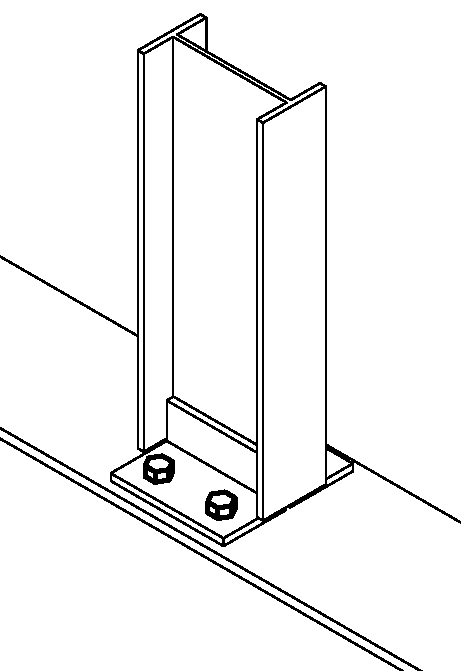
\includegraphics[height=7cm]{PIC/CH06/BBP5}};
\draw[->,line width=2mm,cc0066](0,.5)--++(90:2);
\end{tikzpicture}
\end{figure}
\item Shear --- all bolts have the same shear
\begin{figure}[H]
\begin{tikzpicture}
\node at(0,0){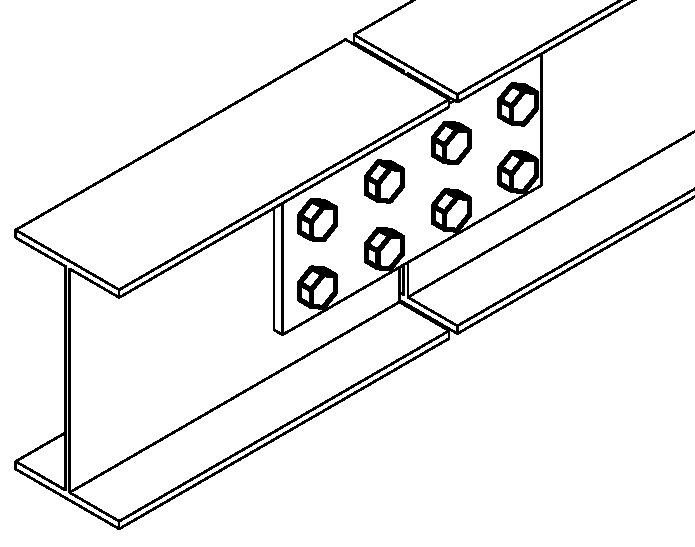
\includegraphics[height=7cm]{PIC/CH06/BBP4}};
\draw[->,line width=2mm,cc0066](-2,-.5)--++(-150:2);
\end{tikzpicture}
\end{figure}
\item Uniform Tension and Shear --- all bolts have the same force
\begin{figure}[H]
\begin{tikzpicture}
\node at(0,0){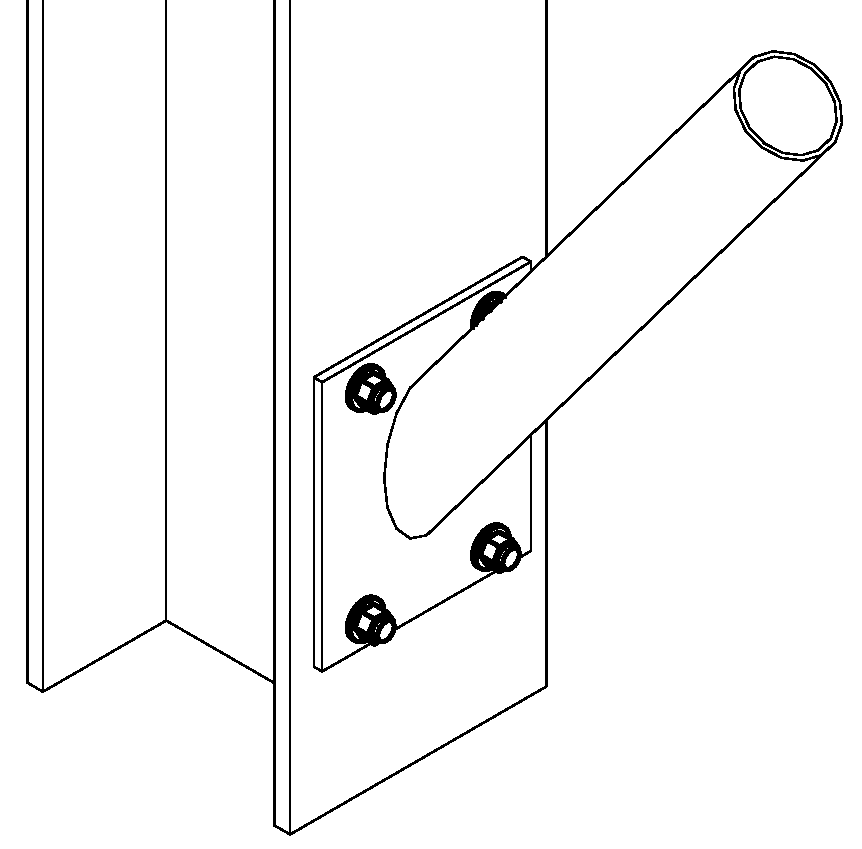
\includegraphics[height=7cm]{PIC/CH06/BBP3}};
\draw[->,line width=2mm,cc0066](1.5,1)--++(45:2);
\end{tikzpicture}
\end{figure}
\item Eccentric Shear
\begin{figure}[H]
\begin{tikzpicture}
\node at(0,0){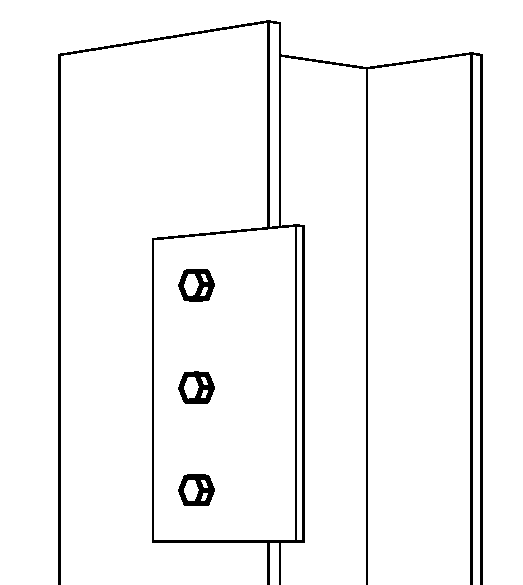
\includegraphics[height=7cm]{PIC/CH06/BBP2}};
\draw[->,line width=2mm,cc0066](1,1)--++(-90:2);
\end{tikzpicture}
\end{figure}
\item Combined Tension and Shear
\begin{figure}[H]
\begin{tikzpicture}
\node at(0,0){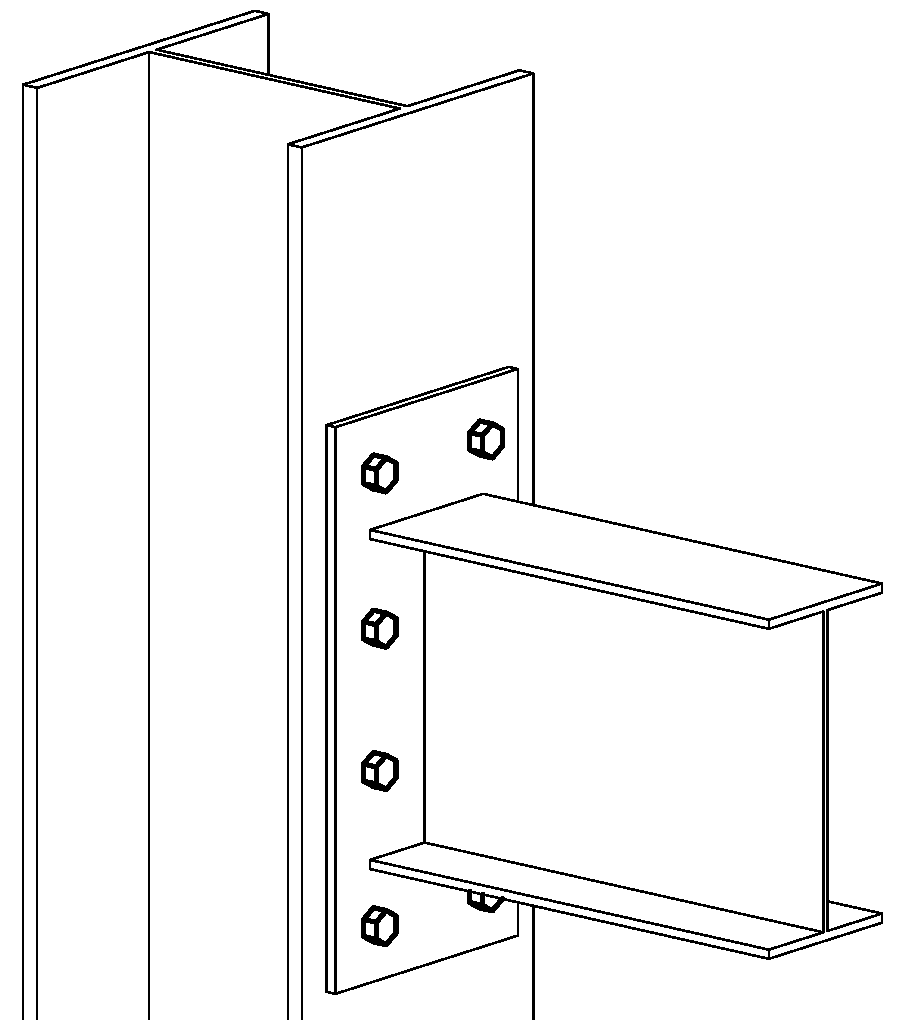
\includegraphics[height=7cm]{PIC/CH06/BBP}};
\draw[->,line width=2mm,cc0066](2,2)--++(-90:2);
\end{tikzpicture}
\end{figure}
\end{itemize}
\section{Connector Types}
Standard connection types are now available in the \href{https://www.scnz.org/techincal-resources/connections-guide/}{Steel Connect}\footnote{\url{https://www.scnz.org/techincal-resources/connections-guide/}}. This means that connections can be specified rapidly using standard notation, and every element of the connection does not need to be designed independently. It is the purpose of this chapter to explain how connections should be designed.
\begin{itemize}
\item \textbf{Pins}\\Used in `zero moment' connections in truss joints.
\item \textbf{Rivets}
\begin{itemize}
\item Hot steel is deformed into shape
\item Shrinks as it cools giving high pretensioning
\item Labour intensive
\end{itemize}
\begin{figure}[H]
\centering
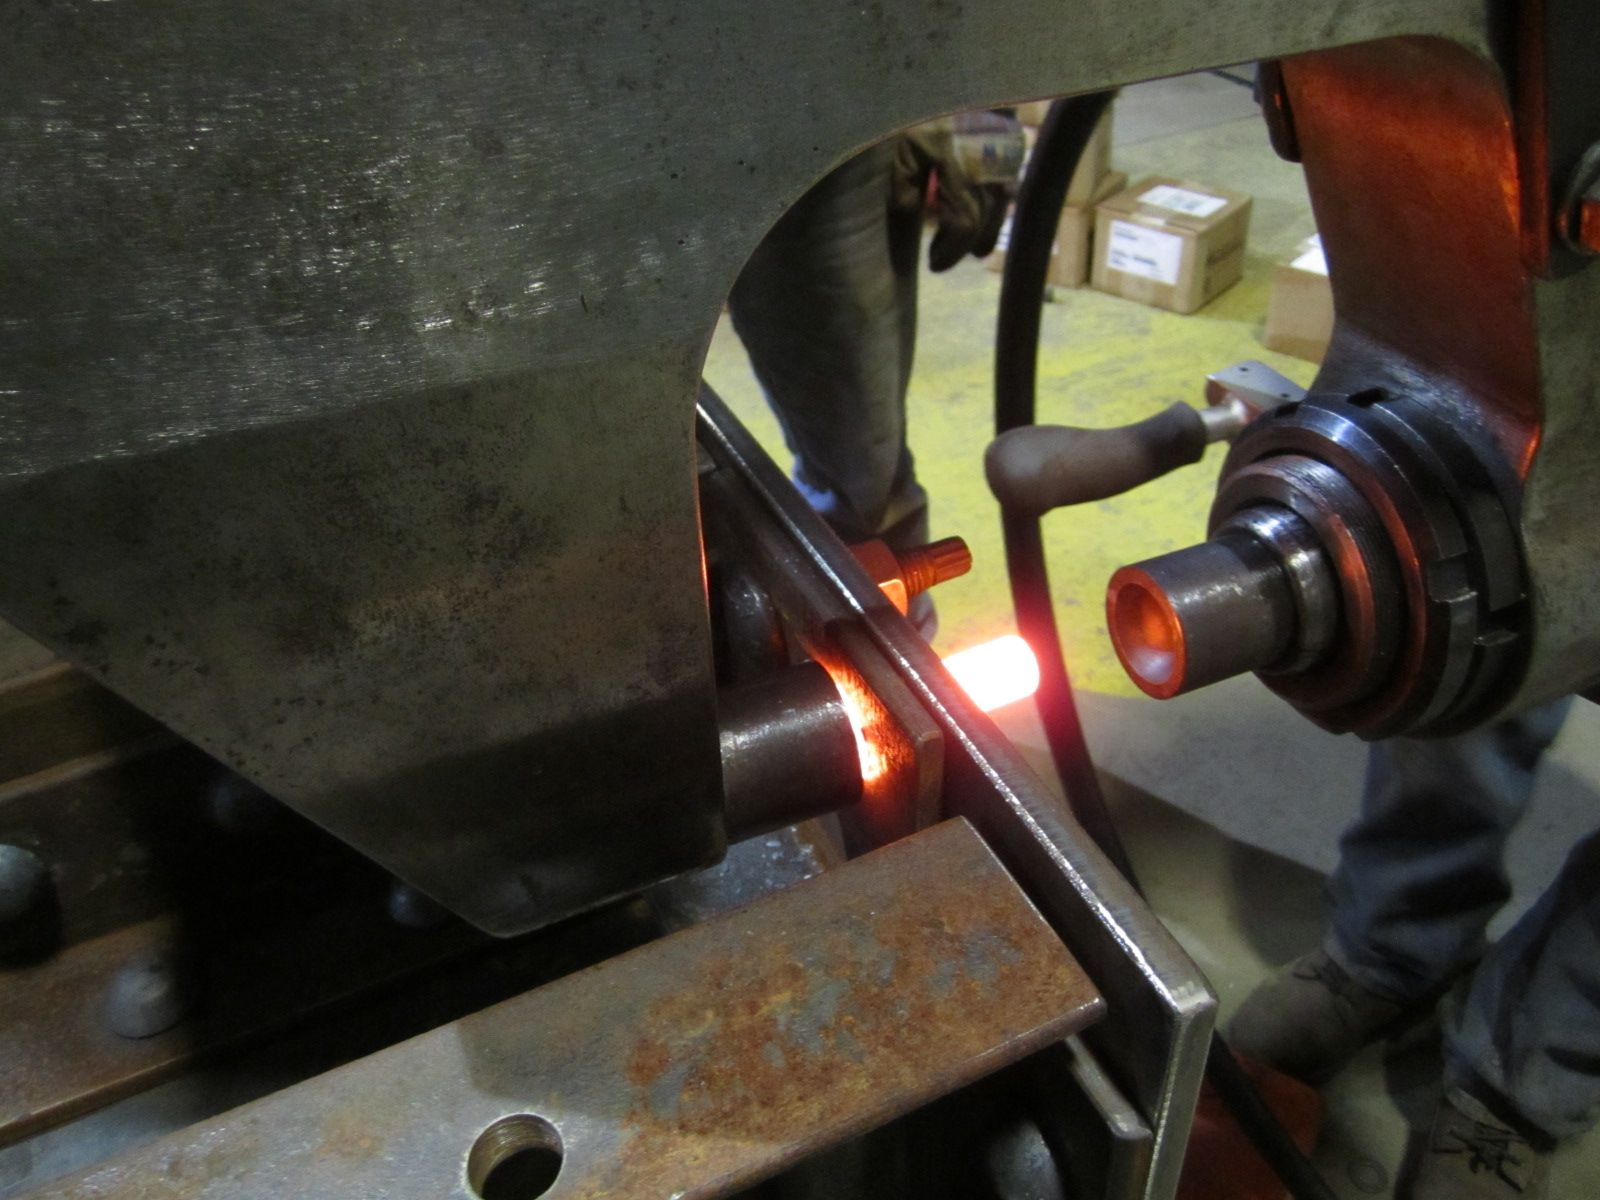
\includegraphics[width=10cm]{PIC/CH06/RI}\caption{Installing a rivet}
\end{figure}
\item \textbf{Bolts}\\
Different head markings also exist depending on the mill, whether it is metric or imperial, and the preference of the mill. It is important to purchase bolts through an SCNZ approved distributor to ensure quality control.

Bolts should be specified according to the grade and standard. (E.g, other grade 8.8 bolts are used for machinery, and these have different properties.) Most structural bolts are galvanised (rather than Zinc coated, or black).
\begin{itemize}
\item Ordinary
\begin{figure}[H]
\centering
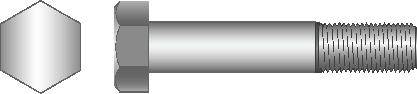
\includegraphics{PIC/CH06/BEXP2}
\end{figure}
\item High Strength (HS)
\begin{figure}[H]
\centering
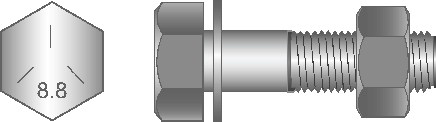
\includegraphics{PIC/CH06/HBEXP2}
\end{figure}
\end{itemize}
\end{itemize}
\section{Bolt Strength}
The types of bolts used in NZ for general structural use are of two types.
\begin{table}[H]
\centering\footnotesize
\begin{tabular}{lllll}
    \toprule
    Grade     & Tensile Strength, $f_{uf}$ & Yield Strength, $f_{yf}$ & Type                   & Standard    \\ \midrule
    Grade 4.6 & \SI{400}{\mpa}             & \SI{240}{\mpa}           & Ordinary or Mild Steel & AS 1111.1   \\
    Grade 8.8 & \SI{830}{\mpa}             & \SI{660}{\mpa}           & High Strength or HSFG  & AS/NZS 1252 \\ \bottomrule
\end{tabular}
\end{table}

HSFG stands for High Strength Friction Grip.

For Grade X.Y bolts, the ultimate strength $f_{uf}$ is about $100\times{}X~\si{\mpa}$, the yield strength $f_{yf}$ is about $10\times{}X\times{}Y~\si{\mpa}$.

Grade 4.6 bolts are mode of low carbon steel (similar to Grade 250 steel) and they are used mostly in secondary members.

Grade 8.8 bolts are make of medium carbon steel using quenching and tempering to enhance the properties. They are used in main framing.

Almost all bolts currently used in Australasia are now made in China.
\section{Bolt Dimension}
The bolt dimensions are shown in \tabref{tab:bolt_dim}.
\begin{table}[H]
\centering\footnotesize\caption{Dimensions of bolts}\label{tab:bolt_dim}
\begin{tabular}{c|cc|ccc|ccc|ccc}
	\toprule
	     &  shank   &  head  & core  & tensile & shank & \multicolumn{3}{c|}{Commercial} & \multicolumn{3}{c}{High Strength} \\
	Type & diameter & height & area  &  area   & area  & width & width &   nut height    & width & width &    nut height     \\
	     &   $E$    &  $C$   & $A_c$ &  $A_s$  & $A_o$ &  $A$  &  $B$  &                 &  $A$  &  $B$  &                   \\ \midrule
	M12  &    12    &   8    & 76.2  &  84.3   &  113  &  18   &  20   &       11        &       &       &                   \\
	M16  &    16    &   11   &  144  &   157   &  201  &  24   &  26   &       15        &  27   &  31   &        17         \\
	M20  &    20    &   13   &  225  &   256   &  314  &  30   &  33   &       18        &  34   &  39   &        21         \\
	M24  &    24    &   16   &  324  &   353   &  452  &  36   &  40   &       22        &  41   &  47   &        24         \\
	M30  &    30    &   20   &  519  &   561   &  706  &  46   &  51   &       26        &  50   &  58   &        31         \\
	M36  &    36    &   24   &  759  &   817   & 1016  &  55   &  61   &       31        &  60   &  69   &        37         \\ \bottomrule
	\multicolumn{12}{l}{All numbers are in \si{\mm} or \si{\mm^2}.}
\end{tabular}
\end{table}
The shank area is computed as $A_o=\pi\dfrac{E^2}{4}$. The core area is computed as $A_c=\pi\dfrac{D^2}{4}$. The tensile area is computed by using pitch diameter which includes threads thus is smaller than $E$ (major diameter) but greater than $D$ (minor diameter).
\begin{figure}[H]
\centering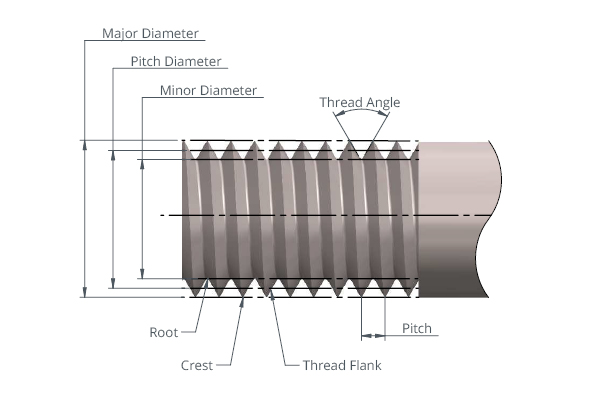
\includegraphics[width=8cm]{PIC/CH06/BDD}
\caption{Bolt diameters (\href{https://www.kelstonactuation.com/imagelibrary/screw-thread-principle.jpg}{\url{https://www.kelstonactuation.com/imagelibrary/screw-thread-principle.jpg}})}
\end{figure}

If not given, the width across corners can be computed according to the width across flats.
\begin{gather}
B\approx\dfrac{2}{\sqrt{3}}A\approx1.1547A.
\end{gather}
\begin{figure}[H]
\centering\begin{tikzpicture}
\node at(0,0){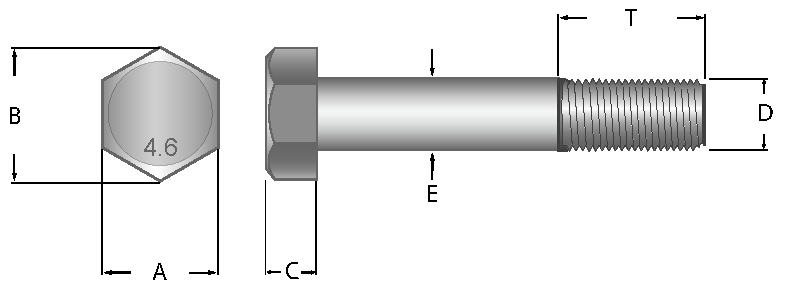
\includegraphics{PIC/CH06/BDIM}};
\node[align=left]at(4,-2){$A$ --- width across flats\\$B$ --- width across corners\\$C$ --- head height\\$D$ --- shank diameter\\$E$ --- core diameter\\$T$ --- thread length};
\end{tikzpicture}
\caption{Bolt dimensions}
\end{figure}

Bolt length is generally measured from the inside of the head of the bolt to the end of the bolt. Some bolts are threaded along their whole length. The minimum length of threaded bolt is shown as follows.
\begin{table}[H]
\centering\footnotesize\caption{Minimum length of thread}
\begin{tabular}{cc}
	\toprule
	          Nominal Length of Bolt, $L$            & Minimum Length of Thread, $T$ \\ \midrule
	            $L\leqslant\SI{125}{mm}$             &            $2D+6$             \\
	$\SI{125}{\mm}\leqslant{}L\leqslant\SI{200}{mm}$ &            $2D+12$            \\
	          $\SI{200}{\mm}\leqslant{}L$            &            $2D+25$            \\ \bottomrule
\end{tabular}
\end{table}

According to \NZSSTEEL{~}, with grip denotes the thickness of materials to be held together, the length of bolt required is
\begin{gather*}
L\geqslant\text{grip}+\text{washer thickness}\times\text{washer number}+\text{nut height},\\
L\leqslant\text{grip}+\text{washer thickness}\times\text{washer number}+\text{thread length}-\SI{3}{\mm}.
\end{gather*}
\begin{figure}[H]
\centering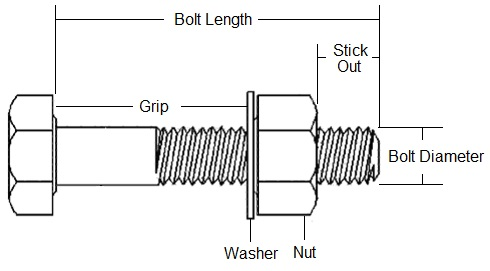
\includegraphics[width=10cm]{PIC/CH06/GRIP}\caption{Definition of grip and washer thickness}
\end{figure}
\section{Installation of Bolts}
Bolts may be installed in two ways:
\begin{itemize}
\item Grade 4.6 Bolts
\begin{itemize}
\item Snug Tightened (4.6/S)
\end{itemize}
\item Grade 8.8 Bolts
\begin{itemize}
\item Snug Tightened (8.8/S)
\item Proof Loaded (8.8/T)
\end{itemize}
\end{itemize}

Snug tightening ensures that the bolt is in full contact with the material. It is defined as `the full effort of one man on a hand wrench tightening the bolt'. It is assumed that the surfaces are clean and flat.

Proof loading may be carried out by any of the following methods.
\begin{enumerate}
\item \textbf{Torque wrench}\\The torque to turn the bolt is measured  giving an indication of the bolt tensile force. It must be calibrated. Clean and flat surfaces are assumed.
\item \textbf{Specified nut rotation method, a.k.a. turn-of-nut method}\\Snug tighten is initially performed. Then the nut is turned a specified amount relative to the bolt as shown.
\begin{figure}[H]
\centering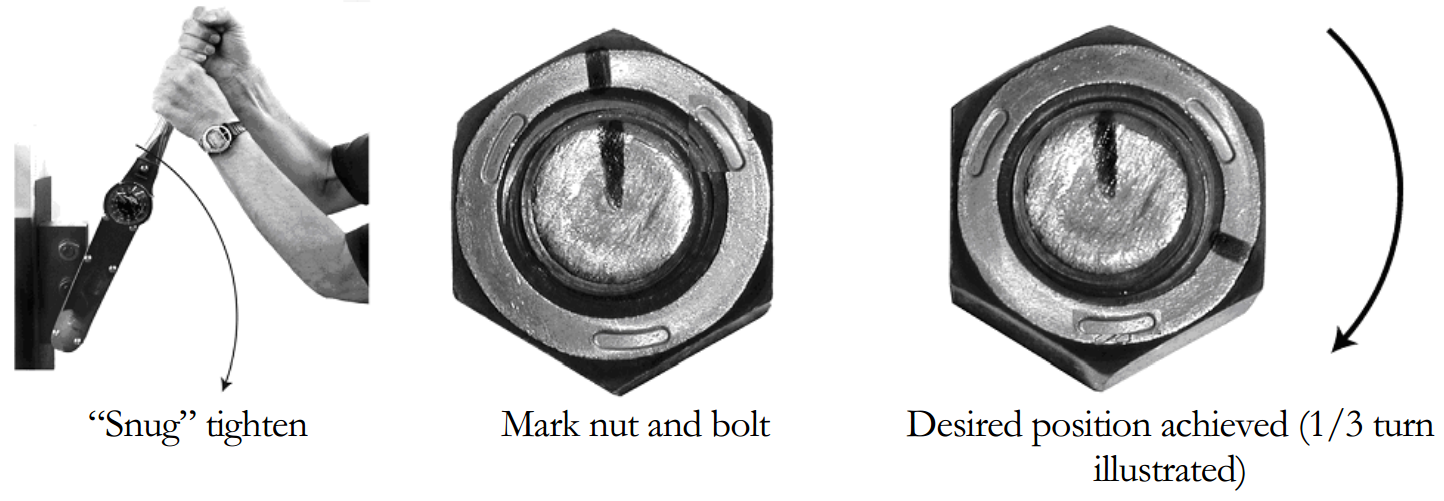
\includegraphics[scale=.25]{PIC/CH06/TON}\caption{Steps of turn-of-nut method}
\end{figure}

The amount of turn required depends on the bolt type. This method is
\begin{itemize}
\item cheap,
\item less dependent on surface conditions, and
\item easy to inspect.
\end{itemize}
\item \textbf{Direct tension indicator (DTI)}\\Tightening on washers with protrusions.
\begin{figure}[H]
\centering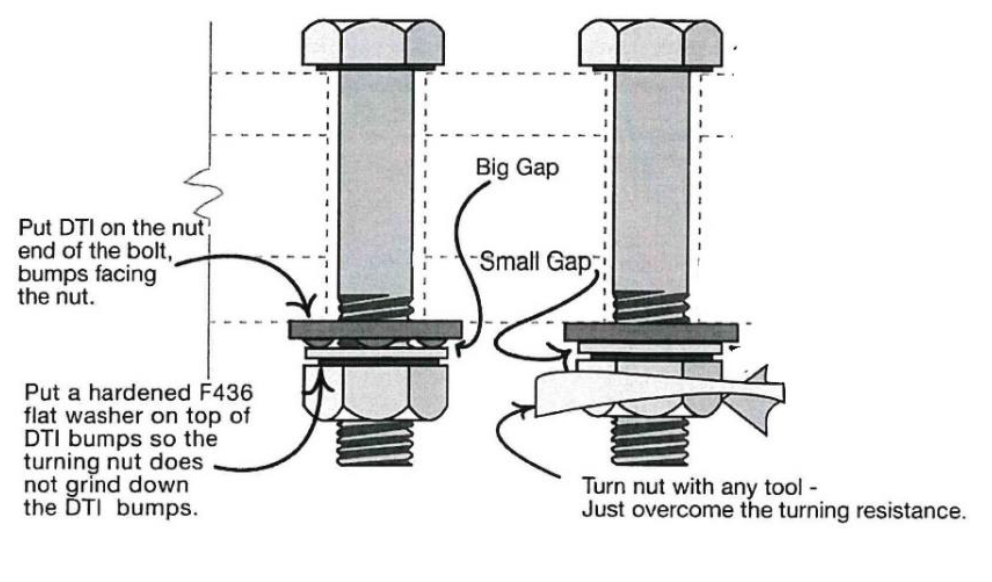
\includegraphics[height=5cm]{PIC/CH06/DTI}
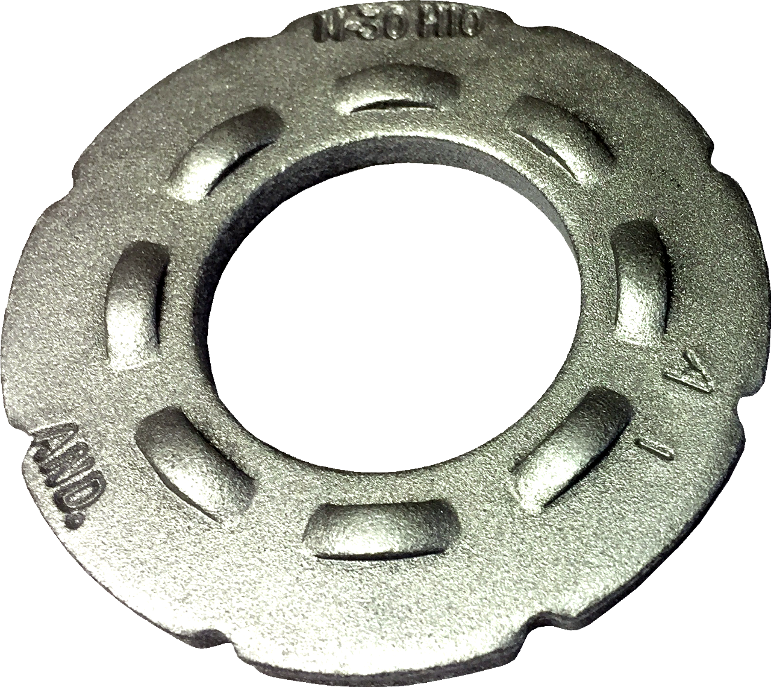
\includegraphics[height=5cm]{PIC/CH06/PRO}
\caption{Direct tension indicator and protrusion}
\end{figure}
This method is
\begin{itemize}
\item less dependent on surface conditions,
\item easy to inspect, and
\item hard to cheat with.
\end{itemize}
\item \textbf{Tension Control Bolts}\\Fracture of bolt end occurs at the notch when proof load is reached.
\begin{figure}[H]
\centering
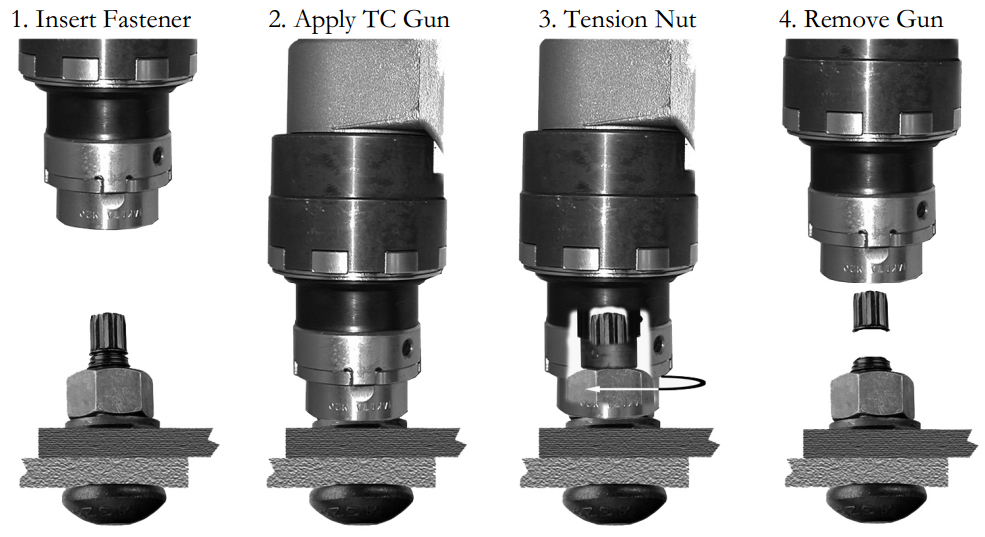
\includegraphics[width=10cm]{PIC/CH06/TCB}\caption{Steps of installing TC bolts}
\end{figure}
This method is
\begin{itemize}
\item fast and easy to inspect, and
\item dependent on surface conditions.
\end{itemize}
\end{enumerate}
All of the proof loading methods above require the bolt to sustain some permanent deformation. Therefore, after proof loading they should \textbf{not} be reused.
\section{Erection Tolerances}
In design of bolts, one shall consider the size of tools used.
\begin{figure}[H]
\centering\footnotesize
\begin{tikzpicture}[scale=1.5]
\draw[dashed](-2,0)--(5.5,0);
\draw[dashed,very thick](-.5,-.25)rectangle++(.5,.5)(.25,-.25)rectangle++(.5,.5);
\draw[very thick](-.5,-.4)rectangle++(1.25,.8)(.75,-.25)rectangle++(.25,.5);
\draw[rounded corners=1.5mm,very thick](1,-.25)to(1.3,-.6)to(1.7,-.6)to(2,-.8)to(2.5,-.8)to(2.5,-1)to(3.5,-1);
\draw[rounded corners=1.5mm,very thick](1,.25)to(1.3,.6)to(1.7,.6)to(2,.8)to(2.5,.8);
\draw[very thick](2.5,-.9)--(2.5,.8)--++(1,0)--(3.5,-1);
\draw[very thick,rounded corners=3mm](3.8,-.6)rectangle(4.2,.4);
\draw[very thick](3.5,.8)to
[rounded corners=6mm](4.5,.8)to
[rounded corners=6mm](5,0)to
[rounded corners=1.5mm](4.7,-.6)to(4.9,-.8)to(4.7,-1)to
[rounded corners=1.5mm](4.5,-.8)to
[rounded corners=4.5mm](4,-1)to(3.5,-.8);
\draw[very thick](3.8,.8)--(3.9,.9)--(4,.9)--(4.1,.8);
\draw[|<->|](-1.5,0)--(-1.5,.8)node[midway,fill=white]{$A$};
\draw[|<->|](-1,0)--(-1,.4)node[midway,fill=white]{$D$};
\draw[|<->|](-.5,-1.5)--++(1.25,0)node[midway,fill=white]{$C$};
\draw[|<->|](.75,-1.5)--++(4.25,0)node[midway,fill=white]{$B$};
\begin{scope}[xshift=6cm,yshift=-1.5cm]
\newcommand{\Bolt}{
\draw[fill=white](-\a,-\a)rectangle(\a,\a);
\draw(-.7*\a,-2.5*\a)rectangle(.7*\a,\a);
\draw(-1.4*\a,\a)rectangle(0,1.8*\a);
\draw(0,\a)rectangle(1.4*\a,1.8*\a);
\draw(-1.4*\a,-\a)rectangle(0,-1.8*\a);
\draw(0,-\a)rectangle(1.4*\a,-1.8*\a);
}
\def\a{.4}\def\b{2}
\draw[pattern=north west lines](0,0)--(2.5,0)arc(0:90:.4)--(.4,.4)--(.4,2.5)arc(0:90:.4)--cycle;
\begin{scope}[xshift=1.3cm,yshift=2mm,scale=.5,rotate=180]
\Bolt
\end{scope}
\begin{scope}[xshift=2mm,yshift=2cm,scale=.5,rotate=90]
\Bolt
\end{scope}
\draw[|<->|](2,2)--(2,.7)node[midway,fill=white]{$E$};
\end{scope}
\end{tikzpicture}\caption{Definition of impact wrench sizes \citep{ASI2016}}
\end{figure}

\begin{table}[H]
\centering\caption{Impact wrench sizes \citep{ASI2016}}
\begin{tabular}{ccc}
	\toprule
	Impact wrench &                                $B$                                &   $A$    \\
	    type      &                             \si{\mm}                              & \si{\mm} \\ \midrule
	   Normal     & \multirow{2}[0]{*}{\parbox{5cm}{\centering{}to 370\\some to 600}} &    55    \\
	    Heavy     &                                                                   &    65    \\ \bottomrule
\end{tabular}
\end{table}
\begin{table}[H]
\centering\caption{Impact wrench sizes \citep{ASI2016}}
\begin{tabular}{ccccccc}
	\toprule
	Nominal  & \multicolumn{3}{c}{Sockets \SI{20}{\mm} drive} & \multicolumn{3}{c}{Sockets \SI{25}{\mm} drive} \\
	  Bolt   &          &          &        Clearance         &          &          &        Clearance         \\
	Diameter &   $C$    &   $D$    &           $E$            &   $C$    &   $D$    &           $E$            \\
	\si{\mm} & \si{\mm} & \si{\mm} &         \si{\mm}         & \si{\mm} & \si{\mm} &         \si{\mm}         \\ \midrule
	   16    &    54    &    48    &            30            &    60    &    58    &            35            \\
	   20    &    57    &    58    &            35            &    63    &    58    &            35            \\
	   24    &    58    &    61    &            35            &    70    &    68    &            40            \\ \bottomrule
\end{tabular}
\end{table}

If extension bar and/or universal joint are used, their dimensions shall also be considered.
\begin{figure}[H]
\centering
\begin{subfigure}{.49\linewidth}\centering
\footnotesize
\begin{tikzpicture}[scale=1]
\draw[dashed](-1,0)--(5,0);
\draw[dashed,thick](-.5,-.25)rectangle++(.5,.5);
\draw[dashed,thick](-.5,-.4)rectangle++(1.25,.8)(3.5,-.25)rectangle++(.5,.5);
\draw[very thick](.25,-.25)to(.25,.25)to[rounded corners=2mm](2.8,.25)to[rounded corners=2mm](3.2,.5)to(4,.5)to(4,-.5)to[rounded corners=2mm](3.2,-.5)to[rounded corners=2mm](2.8,-.25)to(.25,-.25)to cycle;
\draw[|<->|](.25,-1.2)--(4,-1.2)node[midway,fill=white]{\numrange{50}{300}};
\draw[|<->|](4.5,-.5)--(4.5,.5)node[midway,fill=white,right]{\numrange{20}{60}};
\end{tikzpicture}
\caption{Extension bar}
\end{subfigure}\hfill
\begin{subfigure}{.49\linewidth}\centering
\footnotesize
\begin{tikzpicture}[scale=1]
\draw[dashed](-1,0)--(5,0);
\begin{scope}[rotate around={15:(2,0)}]
\draw[dashed](-1,0)--(2,0);
\draw[dashed,thick](-.5,-.4)rectangle++(1.25,.8);
\draw[dashed,thick](-.5,-.25)rectangle++(.5,.5);
\draw[very thick](.25,-.25)rectangle(2,.25);
\end{scope}
\draw[fill=white,very thick](1.5,-.6)to(1.5,.6)to[rounded corners=2mm](2.8,.6)to[rounded corners=2mm](3.2,.4)to(4,.4)to(4,-.4)to[rounded corners=2mm](3.2,-.4)to[rounded corners=2mm](2.8,-.6)to(1.5,-.6)to cycle;
\draw[dashed,thick](3.5,-.25)rectangle++(.5,.5);
\draw[|<->|](1.5,-1.2)--(4,-1.2)node[midway,fill=white]{\numrange{50}{75}};
\draw[|<->|](4.5,-.6)--(4.5,.6)node[midway,fill=white,right]{\numrange{20}{55}};
\draw[|<->|](-.8,0)node[fill=white,above=2mm]{\qtyrange{15}{20}{\degree}}arc(180:195:2.8);
\end{tikzpicture}
\caption{Universal joint}
\end{subfigure}
\caption{Dimension of extension bar and universal joint \citep{ASI2016}}
\end{figure}
\section{Modes of Carrying Shear Force}
\subsection{Shear Planes}
Bolts can be in single (one shear plane) or double (two shear planes) shear as shown below. Threads may be iNcluded (N) or eXcluded (X) from the shear plance (e.g., M20X bolt).
\begin{figure}[H]
\centering
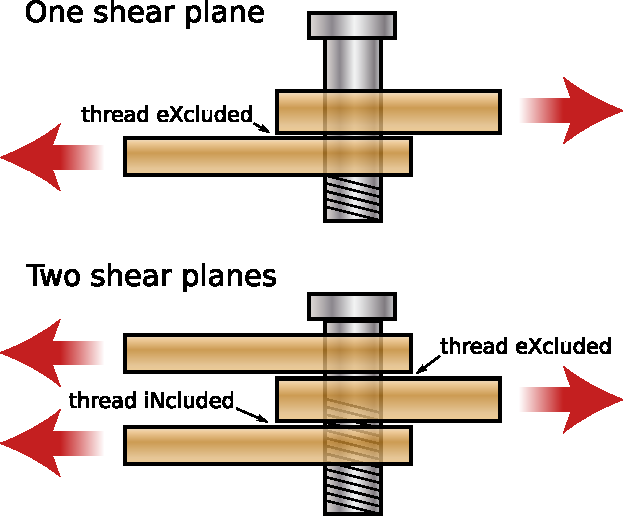
\includegraphics{PIC/CH06/SP}
\caption{Illustration of number of shear planes (\href{https://commons.wikimedia.org/wiki/File:Bolt-in-shear.svg}{\url{https://commons.wikimedia.org/wiki/File:Bolt-in-shear.svg}})}
\end{figure}
\subsection{Snug Tightening}
Shear forces are transferred through \textbf{shear in the bolt}. The following illustration shows two shear planes.
\begin{figure}[H]
\centering
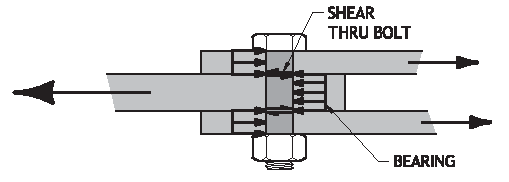
\includegraphics{PIC/CH06/STB}
\caption{Snug tighten bolts \citep{McMullin2018}}
\end{figure}
\subsection{Proof Loading}
This involves tightening the bolt in such a way that it provides a large compressive force on the elements it connects. Force is transferred through \textbf{friction in the plates}. Friction resistance is dependent on both axial (bolt) force $P$ and surface condition (friction coefficient $\mu$). No slip occurs until friction is overcome. When the friction force is overcome, shear force is transferred through both \textbf{bolt shear} and \textbf{friction}.
\begin{figure}[H]
\centering
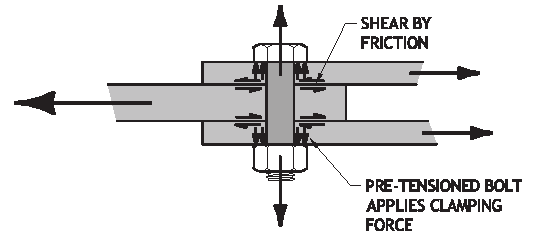
\includegraphics{PIC/CH06/PLB}
\caption{Proof loading bolts \citep{McMullin2018}}
\end{figure}

There are two types of 8.8/T bolts.
\begin{itemize}
\item 8.8/TB --- Tension Bearing
\item 8.8/TF --- Tension Friction
\end{itemize}
These are identical expect that the /TF bolting has treatment of the mating surfaces such that the friction is increased.
\begin{figure}[H]
\centering
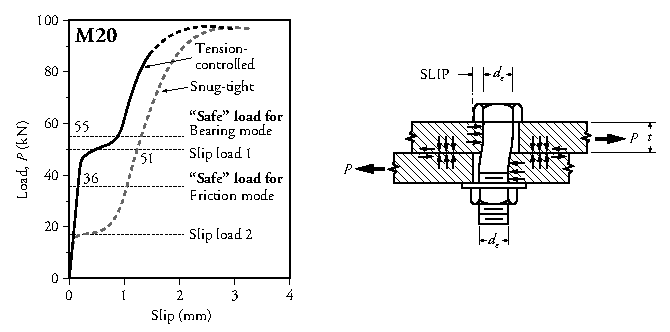
\includegraphics[width=14cm]{PIC/CH06/BLC}
\caption{Behaviour of high-strength structural bolts. Slip load 1 applies to tension-controlled HS structural bolts (i.e., proof loaded bolts) using a slip factor of 0.35. Slip load 2 applies to snug-tight bolts. \citep{Gorenc2015}}
\end{figure}
\section{Minimum Bolt Proof Loads}
It is necessary to tighten the bolt to obtain its `proof load' in order to get the maximum benefit from it.

Proof loading the bolt is tightening it such as it stretches until it applies at least the `proof load', $P_L$. The bolt is then in tension applying a compressive force of $P_L$ to the plates. The compression causes friction between the plates and minimizes deformation.

The minimum proof load for specific bolts is specified in the following table (\NZSSTEEL{Table~15.2.5.1}).
\begin{table}[H]\centering\footnotesize\caption{Minimum Bolt tension for property class 8.8 bolts}
\begin{tabular}{cc}
	\toprule
	Nominal diameter of bolt & Minimum bolt tension (proof load, \si{\kn}) \\ \midrule
	          M16            &                     95                      \\
	          M20            &                     145                     \\
	          M22            &                     180                     \\
	          M24            &                     210                     \\
	          M30            &                     335                     \\
	          M36            &                     490                     \\ \bottomrule
\end{tabular}
\end{table}
It is developed by a mixed consideration of the following:
\begin{itemize}
\item \SI{0.2}{\percent} offset strain
\item \SI{0.5}{\percent} extension under load
\item \SI{70}{\percent} of $f_u$
\end{itemize}
\begin{figure}[H]
\centering\footnotesize
\begin{tikzpicture}
\newdimen\XCoord
\newdimen\YCoord
\draw[->](-1,0)--(10,0)node[below=3mm]{extension ($\si{\percent}$)};
\draw[->](0,-1)--(0,7)node[left=5mm]{stress ($f$)};
\draw[very thick,line join=round,name path=s](0,0)--(1,4)to[out=76,in=180](5,6)to[out=0,in=120](9,4)node{\LARGE\texttimes};
\draw[dashed,name path=e](.3,0)--++(1.6,6.4)node[above,fill=white]{\SI{0.2}{\percent} offset};
\path[name intersections={of=s and e,by=se}];
\path(se);
\pgfgetlastxy{\XCoord}{\YCoord};
\draw[dashed](0,\YCoord)--(se)node[fill=red,inner sep=0,minimum size=2mm,circle]{}--++(1,0)node[align=left,right=1mm,fill=white,anchor=west]{proof loading using \SI{0.2}{\percent} offset strain};
\draw[draw=white,name path=d](1.2,0)node[below]{\SI{0.5}{\percent}}--++(0,6);
\path[name intersections={of=s and d,by=sd}];
\path(sd);
\pgfgetlastxy{\XCoord}{\YCoord};
\draw[dashed](sd)node[fill=red,inner sep=0,minimum size=2mm,circle]{}node[align=left,below right=1mm,fill=white,anchor=north west]{}--(0,\YCoord)(\XCoord,0)--(sd);
\draw[dashed](5,6)node[fill=red,inner sep=0,minimum size=2mm,circle]{}node[align=left,below right=1mm,fill=white,anchor=north west]{}--(0,6)node[left=2mm]{$f_u$};
\draw[dashed,name path=w](0,4.2)--++(6,0)node[fill=white]{proof load using $0.7f_u$};
\path[name intersections={of=s and w,by=sw}];
\path(sw);
\pgfgetlastxy{\XCoord}{\YCoord};
\draw[dashed](sw)node[fill=red,inner sep=0,minimum size=2mm,circle]{}node[align=left,below right=1mm,fill=white,anchor=north west]{}--(0,\YCoord)node[left=2mm]{$0.7f_u$};
\draw[draw=white,name path=t](2.3,0)--++(0,6);
\path[name intersections={of=s and t,by=st}];
\path(st);
\pgfgetlastxy{\XCoord}{\YCoord};
\node at(st)[fill=red,inner sep=0,minimum size=2mm,circle]{}node[align=left,below right=1mm,fill=white,anchor=north west]{};
\draw[dashed](0,\YCoord)--++(6,0)node[fill=white]{proof load using \num{0.5} turn}(\XCoord,0)--(st);
\draw[dashed](.5,0)--++(0,-1);
\draw[-|](0,-1)--(.5,-1)node[below=2mm,midway,align=center]{snug\\tighten};
\draw[-|](.3,-1)--(2.3,-1)node[above=1mm]{\num{0.5}};
\draw[-|](2.3,-1)--(4.3,-1)node[above=1mm]{\num{1}};
\draw[-|](4.3,-1)--(6.3,-1)node[above=1mm]{\num{1.5}}node[right=4mm]{turns from snug tighten};
\end{tikzpicture}
\caption{Proof load}
\end{figure}

The proof load should be as high as possible without the risk of major bolt deformation or failure.
\section{Strengths of Different Bolt Types}
\begin{table}[H]
\centering\footnotesize
\caption{Grade 4.6/S bolted connection strengths for each surface per shear plane}
\begin{tabular}{c|ccc}
	\toprule
	Size &           Shear           &           Shear           &          Axial           \\
	     &        (eXcluded)         &        (iNcluded)         &         Tension          \\
	     & $\phi{}V_{fx}~(\si{\kn})$ & $\phi{}V_{fn}~(\si{\kn})$ & $\phi{}N_{f}~(\si{\kn})$ \\ \midrule
	M12  &           22.4            &           15.1            &            27            \\
	M16  &           39.9            &           28.6            &           50.2           \\
	M20  &           62.3            &           44.6            &           78.4           \\
	M24  &           89.7            &           64.3            &           113            \\
	M30  &            140            &            103            &           180            \\
	M36  &            202            &            151            &           261            \\ \bottomrule
\end{tabular}
\end{table}
\begin{table}[H]
\centering\footnotesize
\caption{Grade 8.8 bolted connection strengths per shear plane}\label{tab:bolt8.8}
\begin{tabular}{c|ccc|cc|ccc}
	\toprule
	Size & \multicolumn{3}{l|}{Strength /S or /T}                                                 & \multicolumn{5}{l}{Serviceability /T}                                                                                      \\ \cline{2-9}
	     &            Shear            &            Shear            &           Axial            &         Proof         &            Axial            & \multicolumn{3}{l}{Shear $\phi{}V_{sf}$ ($\si{\kn}$) for $\mu=0.35$} \\
	     &         (eXcluded)          &         (iNcluded)          &          Tension           &         Load          &           Tension           & Standard &   Short   &                     Long                      \\
	     & $\phi{}V_{fx}$ ($\si{\kn}$) & $\phi{}V_{fn}$ ($\si{\kn}$) & $\phi{}N_{f}$ ($\si{\kn}$) & $N_{tf}$ ($\si{\kn}$) & $\phi{}N_{tf}$ ($\si{\kn}$) & $k_h=1.0$  & $k_h=0.85$ &                   $k_h=0.7$                    \\ \midrule
	M16  &            82.7             &            59.3             &            104             &          95           &            66.5             &   23.3   &   19.8    &                     16.3                      \\
	M20  &             129             &            92.6             &            163             &          145          &            101.5            &   35.5   &   30.2    &                     24.9                      \\
	M24  &             186             &             133             &            234             &          210          &             147             &   51.5   &   43.7    &                     36.0                      \\
	M30  &             291             &             214             &            373             &          335          &            234.5            &   82.1   &   69.8    &                     57.5                      \\
	M36  &             419             &             312             &            542             &          490          &             343             &  120.1   &   102.0   &                     84.0                      \\ \bottomrule
\end{tabular}
\end{table}
\section{Strength Design}
The strength reduction factor $\phi$ shall be taken as follows for bolted connections.
\begin{table}[ht]
\centering\caption{Strength reduction factor for bolted connections}
\begin{tabular}{llcl}
	\toprule
	Design capacity                          & Section               &  $\phi$   & Location      \\ \midrule
	(ULS) bolt in shear                      & \NZSSTEEL{\S~9.3.2.1} & \num{0.8} & in bolt       \\
	(ULS) bolt in tension                    & \NZSSTEEL{\S~9.3.2.2} & \num{0.8} & in bolt       \\
	(ULS) bolt in combined shear and tension & \NZSSTEEL{\S~9.3.2.3} & \num{0.8} & in bolt       \\
	(ULS) ply in bearing                     & \NZSSTEEL{\S~9.3.2.4} & \num{0.9} & on steel      \\
	(ULS) bolt group                         & \NZSSTEEL{\S~9.4}     & \num{0.8} & in bolt       \\
	(SLS) friction type                      & \NZSSTEEL{\S~9.3.3}   & \num{0.7} & between steel \\ \bottomrule
	                                         &                       &           &
\end{tabular}
\end{table}
\subsection{Connection Behaviour}
Load is initially carried by only one bolt due to inaccurate hole placement. After it yields, other bolts can carry loads. The concept is illustrated in the following figure. \textbf{The shear force in a connection is often assumed to be carried equally by each of the bolts.} Bearing connections are used when slip is not important.
\begin{figure}[H]
\centering\begin{tikzpicture}
\def\a{.4}\def\b{2}
\newcommand{\Bolt}{
\draw[fill=white](-\a,-\a)rectangle(\a,\a);
\draw(-.7*\a,-2.5*\a)rectangle(.7*\a,\a);
\draw(-1.4*\a,\a)rectangle(0,1.8*\a);
\draw(0,\a)rectangle(1.4*\a,1.8*\a);
\draw(-1.4*\a,-\a)rectangle(0,-1.8*\a);
\draw(0,-\a)rectangle(1.4*\a,-1.8*\a);
}
\draw(-\b,0)rectangle(1.5*\b,\a);
\draw(-1.5*\b,0)rectangle(\b,-\a);
\draw[->](1.6*\b,.5*\a)--++(1,0)node[right=3mm]{$N^*$};
\draw[->](-1.6*\b,-.5*\a)--++(-1,0)node[left=3mm]{$N^*$};
\node[anchor=center]at(0,1.2){Initially left bolt is loaded.};
\setstructmech{convention=direction}
\begin{scope}[xshift=-.5cm]
\Bolt
\UDL{-.7*\a,0}{-.7*\a,\a}{.4}
\UDL{.7*\a,0}{.7*\a,-\a}{.4}
\end{scope}
\begin{scope}[xshift=1cm]
\Bolt
\end{scope}
\begin{scope}[yshift=-3cm]
\draw(-\b,0)rectangle(1.5*\b,\a);
\draw(-1.5*\b,0)rectangle(\b,-\a);
\draw[->](1.6*\b,.5*\a)--++(1,0)node[right=3mm]{$N^*$};
\draw[->](-1.6*\b,-.5*\a)--++(-1,0)node[left=3mm]{$N^*$};
\node[anchor=center]at(0,1.2){After left bolt yields, right bolt can also carry load.};
\begin{scope}[xshift=-.5cm]
\Bolt
\UDL{-.7*\a,0}{-.7*\a,\a}{.4}
\UDL{.7*\a,0}{.7*\a,-\a}{.4}
\end{scope}
\begin{scope}[xshift=1cm]
\Bolt
\UDL{-.7*\a,0}{-.7*\a,\a}{.4}
\UDL{.7*\a,0}{.7*\a,-\a}{.4}
\end{scope}
\end{scope}
\end{tikzpicture}
\end{figure}

\begin{figure}[H]
\centering
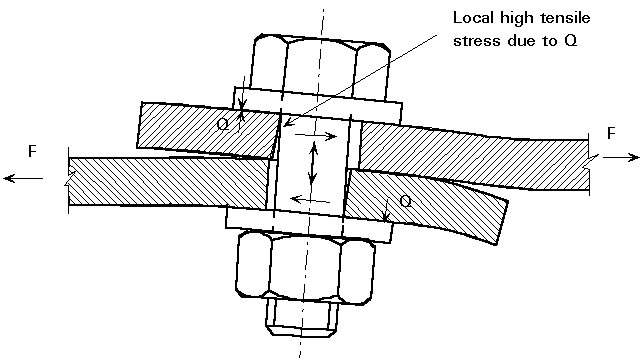
\includegraphics[scale=.5]{PIC/CH06/BD}
\caption{Actual deformation of bolted single shear tension connection (\href{http://fgg-web.fgg.uni-lj.si/~/pmoze/esdep/master/wg11/l0310.htm}{\url{http://fgg-web.fgg.uni-lj.si/~/pmoze/esdep/master/wg11/l0310.htm}})}
\end{figure}
\subsection{Yield on Plate Gross Area}
This was discussed in \S~\ref{sec:tension}, see \eqsref{eq:tension_gross}.
\subsection{Fracture on Plate Net Area}
This was discussed in \S~\ref{sec:tension}, see \eqsref{eq:tension_net}.
\subsection{Bolt Shear Failure}
The design strength of bolts in shear is affected by the ultimate shear strength of the steel, the bolt net area, the mode by which shear force is carried, the distribution of force among bolts in a connection.

The core area of the bolt, $A_c$, is used when the shear plane passes through the threaded area. $A_c$ is given in \tabref{tab:bolt_dim} and it is often $0.75A_o$ to $0.8A_o$ where $A_o$ is the shank area.
\begin{figure}[H]
\centering
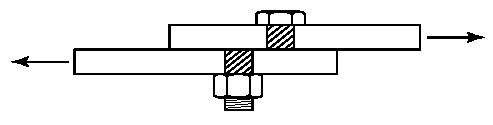
\includegraphics[scale=1.2]{PIC/CH06/BSF}\caption{Bolt shear failure}
\end{figure}

Experiments show that
\begin{itemize}
\item the ultimate shear stress in bolts is $\tau_{u}\approx0.62f_u$. The value of \num{0.62} is close to $\tau_y/f_y=1/\sqrt{3}=0.577$ given by von Mises yielding criterion of steel;
\item in connections which are more than $\SI{1300}{\mm}$ long, the forces are not shared evenly over all bolts, so bolts should be designed to resist a greater shear force;
\item a bolt in double shear can carry twice as much shear force as one in single shear (as long as they both have the same shear area).
\end{itemize}

The design shear force $V^*_f$ for a bolt shall satisfy (\NZSSTEEL{\S~9.3.2.1})
\begin{gather}
V^*_f\leqslant\phi{}V_f=\phi0.62k_rf_{uf}\left(n_nA_c+n_xA_o\right),
\end{gather}
where
\begin{conditions}
\phi&strength reduction factor, \num{0.8}\\
k_r&reduction factor\\
f_{uf}&minimum tensile strength of the bolt\\
n_n&number of shear planes \textbf{iNcluding} threads intercepting the shear plane\\
A_c&minor diameter area of the bolt\\
n_x&number of shear planes \textbf{eXcluding} threads intercepting the shear plane\\
A_o&nominal plain shank area of the bolt
\end{conditions}
The factor $k_r$ shall be taken as \num{1.0} for lap connections with lengths up to $\SI{300}{\mm}$ and \num{0.75} for lap connections with lengths over $\SI{1300}{\mm}$. Linear interpolation shall be used for lengths between $\SI{300}{\mm}$ and $\SI{1300}{\mm}$. For all other connections, $k_r=1.0$.

It can be alternatively expressed as
\begin{gather}
V_f=n_nV_{fn}+n_xV_{fx},
\end{gather}
with
\begin{gather}
V_{fn}=0.62k_rf_{uf}A_c,\\
V_{fx}=0.62k_rf_{uf}A_o.
\end{gather}
The nominal capacity $V_f$ is the summation of capacities of all shear planes of two types.
\subsection{Plate Bearing and Tearing Failure Beside Bolts}
For bolts to develop their strength, the material around bolts must be strong enough to resist bolt forces. That is, the plate material should not fail in \textbf{bearing}, and if bolts are near the side or edge of the plate or if bolt holes near other holes, then the possibility of \textbf{plate yielding or facture} should be considered in the assessment of the maximum force that the bolt can carry. Different values of edge distance are given for holes of different sizes and shapes.

\textbf{Bearing} causes deformation and elongation of the plate beside the hole. Strength loss will occur due to plate fracture as discussed later.
\begin{figure}[H]
\centering
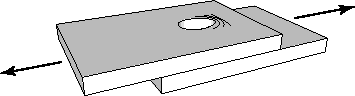
\includegraphics[width=8cm]{PIC/CH06/BBEAR}\caption{Bearing failure}
\end{figure}

Codes generally have an allowable resistance, $R_n$, greater than $A_bf_u$. This is due to the following reasons.
\begin{itemize}
\item The part of the plate in bearing is subject to compressive force.
\begin{itemize}
\item The ultimate strength $f_u$ is found from a tension test.
\item In compression, the strength is larger (see \figref{fig:steel_response}).
\end{itemize}
\item Swelling of the plate (Poisson's effect) causes an increase in bolt compressive forces. This cause a triaxial loaded state which leads to higher strength.
\item Collapse does not occur as a result of bearing failure.
\end{itemize}

If the strength of bolt is less than the strength of plate, then design for bearing of the bolt should be carried out.

\textbf{Bolt tear out failure} occurs when the distance between bolt hole and the edge of plate, or the distance between adjacent bolt holes in the line of force is small.
\begin{figure}[H]
\centering
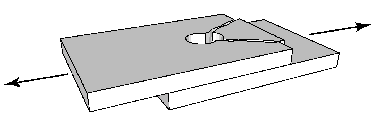
\includegraphics[width=8cm]{PIC/CH06/BTEAR}\caption{Tear out failure}
\end{figure}

\textbf{Edge failure} due to bolt loading in a direction which is not in the line of force should also be considered.
\begin{figure}[H]
\centering
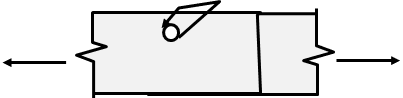
\includegraphics[width=8cm]{PIC/CH06/SF}\caption{Edge failure of plate}
\end{figure}

\textbf{Oversize holes} may require special edge distance and bearing design because loading may be more concentrated.

According to \NZSSTEEL{\S~9.3.2.4.1}, a ply subject to a design bearing force $V^*_b$ due to bolt in shear shall satisfy
\begin{gather}
V^*_b\leqslant{}C_1\phi{}V_b.
\end{gather}
For \textbf{non-seismic}  design, $C_1=1.0$. For seismic design, $C_1<1.0$. It could be as low as \num{0.6} for seismic design according to \NZSSTEEL{\S~12.9.4.3}. Also, using $C_1=0.6$ is a good default for all NZ connections as it will reduce the bolt hole deformation, and the possibility of significantly pinched hysteretic behaviour causing large impacts during earthquake shaking. The nominal bearing capacity $V_b$ of a ply shall be the \textbf{smaller} of the following two.
\begin{enumerate}
\item \textbf{Ply bearing failure beside bolt (Eq. 9.3.2.4(1))}
\begin{gather}
V_b=3.2d_ft_pf_{up},
\end{gather}
where
\begin{conditions}
d_f&bolt diameter\\
t_p&ply thickness\\
f_{up}&ply ultimate strength
\end{conditions}
\item \textbf{Bolt tearing out failure (Eq. 9.3.2.4(2))}
\begin{gather}
V_b=a_et_pf_{up},
\end{gather}
where
\begin{conditions}
a_e&minimum distance from hole edge to edge of ply in direction of force plus half of $d_f$
\end{conditions}
\begin{figure}[H]
\centering\footnotesize
\begin{tikzpicture}
\draw(-1,-2)rectangle(4,2);
\draw(.6,0)circle(4mm);
\draw[fill=black](.5,0)circle(3mm);
\draw[|<->|](-1,.7)--(.2,.7)node[midway,fill=white,align=center,above=2mm]{$e$, clear\\distance};
\draw[|<->|](-1,-.7)--(.5,-.7)node[midway,fill=white]{$a_e$};
\draw[|<->|](-1,-1)--(.6,-1)node[midway,below=2mm]{$e+d_h/2$};
\draw[->,line width=.8mm](5,0)--++(1,0)node[right]{$N^*$};
\node[align=left,anchor=west]at(5,-1.2){$a_e=e+d_f/2$\\Note $d_f\neq{}d_h$};
\end{tikzpicture}\caption{Illustration of $a_e$}
\end{figure}
\end{enumerate}

The following requirements shall be met to avoid potential failure modes.
\begin{figure}[H]
\centering\footnotesize
\begin{tikzpicture}
\draw(0,-1.5)rectangle(6,1.5);
\draw(1,0)circle(2mm);
\draw[dashed](1,0)circle(10mm);
\draw(3,0)circle(2mm);
\draw(5,0)circle(2mm);
\draw[|<->|](3,0)--++(2,0)node[midway,fill=white]{$s$};
\draw[|<->|](0,0)--++(.8,0)node[midway,fill=white]{$e$};
\end{tikzpicture}\caption{Illustration of minimum pitch $s$ and edge distance $e$}
\end{figure}
\begin{enumerate}
\item \textbf{Bolt spacing failure}\\
\NZSSTEEL{\S~9.6.1} requires the minimum pitch $s$ (the distance between centres of bolt holes) shall be at least $2.5d_f$.
\begin{gather}
s\geqslant2.5d_f.
\end{gather}
\item \textbf{Bolt side failure}\\
\NZSSTEEL{\S~9.6.2.1} defines the edge distance to be the distance from the nearer edge of the hole to the physical edge of the plate or rolled section \textbf{plus} half of $d_f$. The edge distance $a_e=e+d_f/2$ shall meet the following minimum values for different cases:
\begin{itemize}
\item $1.75d_f$ for sheared or hand flame cut edge
\item $1.5d_f$ for rolled plate, flat bar or section: machine flame cut, sawn or planed edge
\item $1.25d_f$ for rolled edge of a rolled flat bar or section
\end{itemize}
\item \textbf{Corrosion between plates}\\
\NZSSTEEL{\S~9.6.3} requires the maximum distance between centres of holes shall be the smaller of $15t_p$ and $\SI{200}{\mm}$.
\begin{gather}
s\leqslant\min\left(15t_p,~\SI{200}{\mm}\right).
\end{gather}
\end{enumerate}
\subsection{Block Shear Failure}\label{sec:block_failure}
Block shear/tearing failure is not explicitly considered in \NZSSTEEL{}. However, it has caused connection failures in the past.
\begin{figure}[H]
\centering\footnotesize
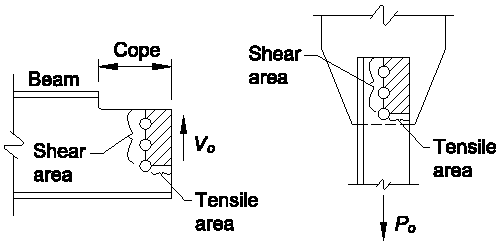
\includegraphics[scale=1.5]{PIC/CH06/BLOCK}\caption{Illustration of block shear failure}
\end{figure}

Similar to tension members, in this course, we the following expression to determine capacity when tension stress is uniform.
\begin{gather}\label{eq:block_shear}
N^*\leqslant\phi0.95\left(0.6A_{ev}f_u+A_{nt}f_u\right),
\end{gather}
where
\begin{conditions}
\phi&strength reduction factor, \num{0.9}\\
A_{ev}&effective area subject to shear\\
A_{nt}&net area subject to tension
\end{conditions}

The effective shear area is taken as the average of net and gross shear areas.
\begin{gather}
A_{ev}=\dfrac{1}{2}\left(A_{gv}+A_{nv}\right),
\end{gather}
where $A_{nv}$ and $A_{gv}$ have been introduced previously and are also illustrated in the following figure.
\begin{figure}[H]
\centering\footnotesize
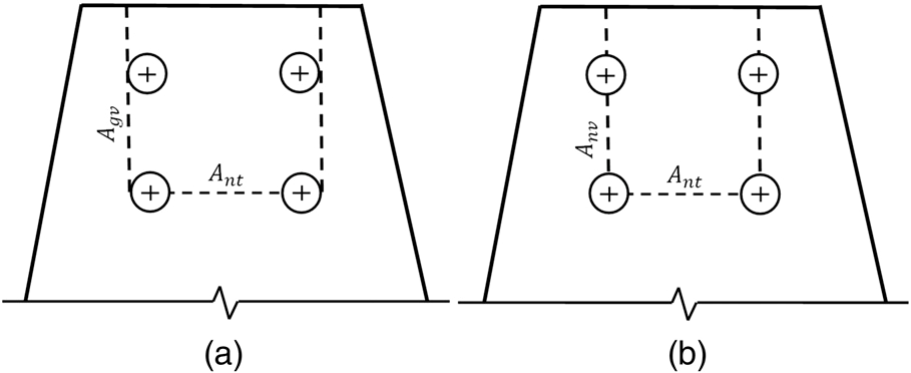
\includegraphics[width=12cm]{PIC/CH06/TB}
\caption{Definition of net and gross areas}
\end{figure}
\begin{figure}[H]
\centering\footnotesize
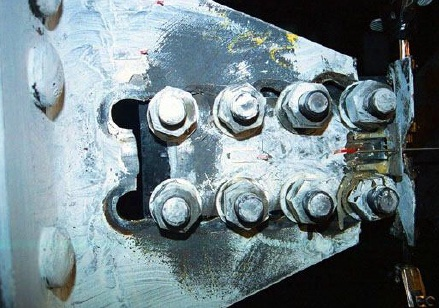
\includegraphics[scale=.8]{PIC/CH06/BTOF}
\caption{Failure surface of block shear/tear (\href{https://m2ukblog.wordpress.com/2016/05/28/block-shear-failure-in-tension-members/}{\url{https://m2ukblog.wordpress.com/2016/05/28/block-shear-failure-in-tension-members/}})}
\end{figure}
\subsection{Bolt Tension Failure}
\begin{figure}[H]
\centering
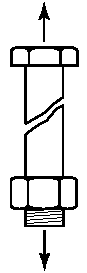
\includegraphics[angle=-90,width=8cm]{PIC/CH06/BTF}\caption{Bolt tension failure}
\end{figure}
\NZSSTEEL{9.3.2.2} requires
\begin{gather}
N^*_{tf}\leqslant\phi{}N_{tf}=\phi{}A_sf_{uf},
\end{gather}
where
\begin{conditions}
\phi&strength reduction factor, \num{0.8}\\
N_{tf}&nominal tension capacity of a bolt\\
A_s&tensile stress area of a bolt\\
f_{uf}&minimum tensile strength of a bolt
\end{conditions}
\subsection{Bolt Combined Failure}\label{sec:bolt_combined}
\NZSSTEEL{9.3.2.3} requires
\begin{gather}
\left(\dfrac{V^*_{f}}{\phi{}V_{f}}\right)^2+\left(\dfrac{N^*_{tf}}{\phi{}N_{tf}}\right)^2\leqslant1.0.
\end{gather}
\begin{figure}[H]
\centering\footnotesize
\begin{tikzpicture}
\begin{axis}[
width=7cm,height=7cm,
axis x line=middle,
axis y line=middle,
axis equal,
xlabel=$\dfrac{N^*_{tf}}{\phi{}N_{tf}}$,
ylabel=$\dfrac{V^*_{f}}{\phi{}V_{f}}$,
x label style={at={(axis description cs:0.5,-0.05)},anchor=north},
y label style={at={(axis description cs:-0.15,.5)},anchor=south},
xmin=-.1,
ymin=-.1,
xmax=1.1,
ymax=1.1,
]
\addplot[domain=0:.72,samples=100,line width=.8mm]({x},{(1-x^2)^(.5)});
\addplot[domain=0:.72,samples=100,line width=.8mm]({(1-x^2)^(.5)},{x});
\addplot[domain=0:1,samples=2,dashed]({x},{1-x});
\end{axis}
\end{tikzpicture}\caption{Envelop of axial force versus shear}
\end{figure}
\subsection{Bending Failure of Bolts}
Bending failure is not usually aa problem expect for very long bolts. Standard methods can be used.
\begin{figure}[H]
\centering
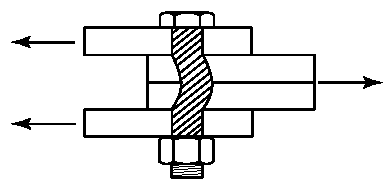
\includegraphics{PIC/CH06/BBF}\caption{Bending failure of bolts}
\end{figure}
\subsection{Fatigue Failure of Bolts}
The strength of bolts is reduced by fatigue and methods are available for design.
\subsection{Prying}
Prying forces, $Q$, act on the flange of an I or T section when the web is in tension and the flange stiffness is moderate. The prying forces cause a) larger bolt forces, and b) greater flange moments. The actual size of $Q$ is difficult to assess. However, it can be significant. A design method is described by \citet{Salmon2009}.
\begin{figure}[H]
\centering
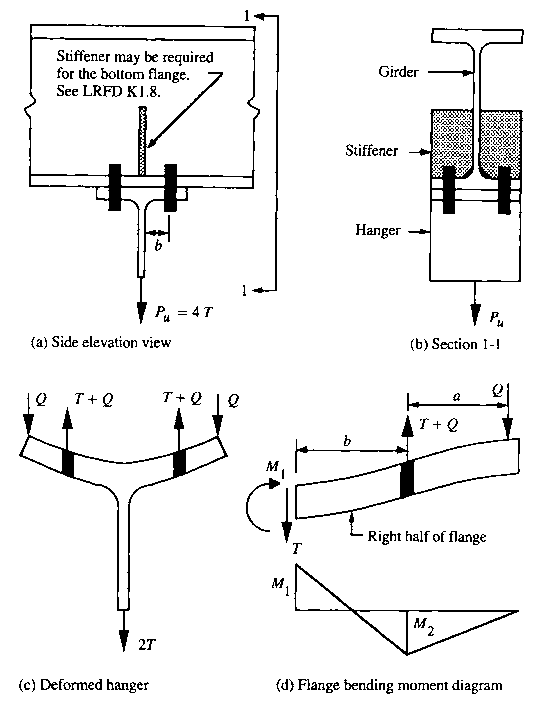
\includegraphics[scale=1]{PIC/CH06/PRY3}
\caption{T section hanger connection \citep{Smith1996}}
\end{figure}
\begin{figure}[H]
\centering
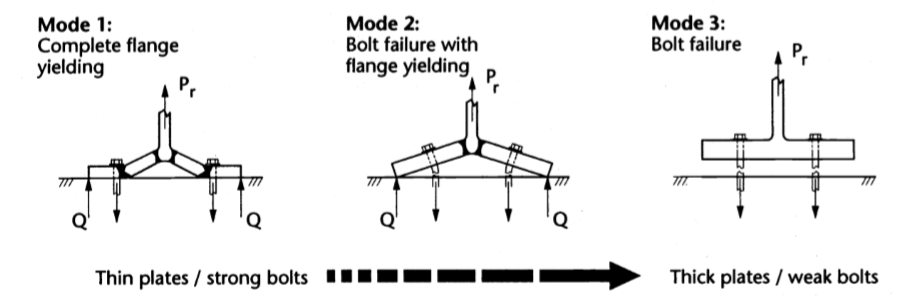
\includegraphics[width=14cm]{PIC/CH06/PRY}
\caption{Prying failure modes (\href{https://www.structures-simplified.com/2020/08/why-prying-force-is-important.html}{\url{https://www.structures-simplified.com/2020/08/why-prying-force-is-important.html}})}
\end{figure}

\begin{exmp}\href{run:./WORKSHEET/CH06/EX6.DABC.sm}{Worksheet} Double Angle Bolted Connection

Assume connection length is smaller than $\SI{300}{\mm}$, find the lightest pair of Grade 300 angles with long legs back-to-back to carry $N^*=\SI{320}{\kn}$. Using bearing type M16 Grade 8.8N bolts, a bolt spacing $s=\SI{40}{\mm}$ and an end distance of $\SI{30}{\mm}$.
\begin{figure}[H]
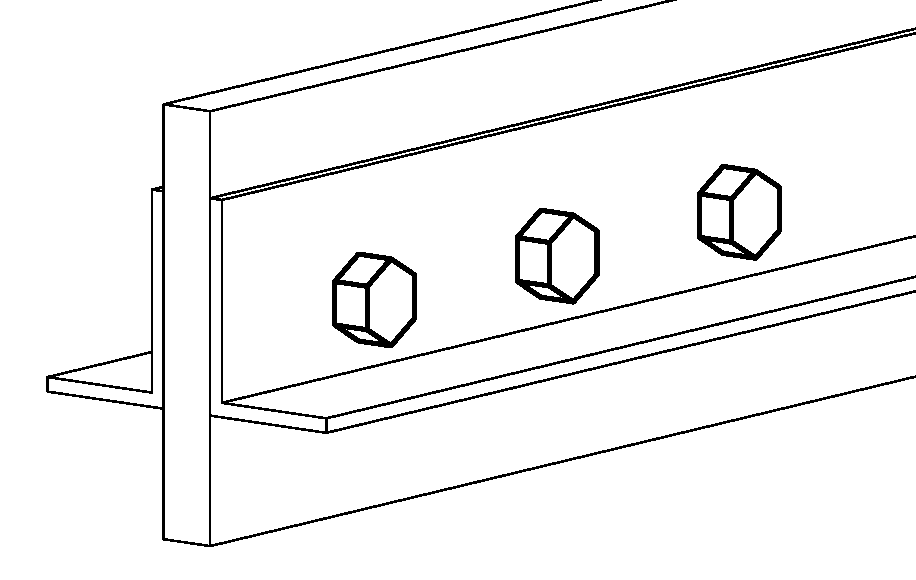
\includegraphics[width=8cm]{PIC/CH06/DAC}
\end{figure}
\end{exmp}
\begin{solution}
\begin{enumerate}
\item Determine the number of bolts required.\\
The connection length is smaller than $\SI{300}{\mm}$, $k_r=1.0$. The shear capacity per bolt shall be calculated as
\begin{align*}
\phi{}V_f&=\phi0.62k_rf_{uf}\left(n_nA_c+n_xA_o\right)\\
&=\phi0.62k_rf_{uf}n_nA_c\\
&=0.8\times0.62\times1\times\SI{830}{\mpa}\times2\times\SI{144}{\mm^2}\\
&=\SI{118.6}{\kn}.
\end{align*}
The above value can also be computed as $2\times\SI{59.3}{\kn}=\SI{118.6}{\kn}$, see \tabref{tab:bolt8.8}.

The number of bolts is then
\begin{gather*}
n\geqslant\dfrac{N^*}{\phi{}V_f}=2.70.
\end{gather*}
Thus use \num{3} bolts.
\item Check bearing on angle.\\
The bearing force on each bolt is
\begin{gather*}
V^*_b=\dfrac{\SI{320}{\kn}}{3\times2}=\SI{53.3}{\kn}.
\end{gather*}
The bearing capacity of each bolt shall be greater than force,
\begin{gather*}
\phi3.2d_ft_pf_{up}=\phi{}V_b\geqslant{}V^*_b
\end{gather*}
This leads to
\begin{gather*}
t_p\geqslant\dfrac{\SI{53.3}{\kn}}{0.9\times3.2\times\SI{16}{\mm}\times\SI{440}{\mpa}}=\SI{2.63}{\mm}.
\end{gather*}
\item Check end distance.
\begin{gather*}
\phi{}a_et_pf_{up}=\phi{}V_b\geqslant{}V^*_b.
\end{gather*}
This gives
\begin{gather*}
t_p\geqslant{}\dfrac{\SI{53.3}{\kn}}{0.9\times\SI{29}{\mm}\times\SI{440}{\mpa}}=\SI{4.64}{\mm}.
\end{gather*}
\item Check yielding on gross area.\\
Assume $f_y=\SI{320}{\mpa}$ and $f_u=\SI{440}{\mpa}$,
\begin{gather*}
A_g\geqslant\dfrac{1}{2}\dfrac{N^*}{\phi{}f_y}=\dfrac{1}{2}\dfrac{\SI{320}{\kn}}{0.9\times\SI{320}{\mpa}}=\SI{555.6}{\mm^2}.
\end{gather*}
\item Check fracture on net area.\\
It can be looked up $k_{te}=1.0$.
\begin{gather*}
A_e\geqslant\dfrac{1}{2}\dfrac{N^*}{\phi{}0.85k_{te}f_u}=\dfrac{1}{2}\dfrac{\SI{320}{\kn}}{0.9\times0.85\times1\times\SI{440}{\mpa}}=\SI{475.3}{\mm^2}.
\end{gather*}
The gross area should satisfy
\begin{gather*}
A_g\geqslant\SI{475.3}{\mm^2}+18t_p.
\end{gather*}
\item Check edge distance in any direction.
\begin{enumerate}
\item The minimum distance:
\begin{gather*}
L_{e,min}=1.25d_f=1.25\times\SI{16}{\mm}=\SI{20}{\mm}.
\end{gather*}
This is equivalent to $\SI{21}{\mm}$ to bolt centre.
\item The maximum distance:
\begin{align*}
L_{e,max}=\min\left(\SI{150}{\mm},~12t_p\right)=\SI{60}{\mm},
\end{align*}
assuming $t_p=\SI{5}{\mm}$.
\end{enumerate}
\end{enumerate}

A quick summary, the desired section shall meet the following requirements:
\begin{enumerate}
\item $t_p\geqslant\SI{4.64}{\mm}$
\item $A_g\geqslant\SI{555.6}{\mm^2}$
\item $A_g\geqslant\SI{475.3}{\mm^2}+18t_p$
\item $\SI{21}{\mm}\leqslant\text{Edge Distance}\leqslant\SI{60}{\mm}$
\end{enumerate}

Try 65\texttimes50\texttimes5UA, $A_g=\SI{512}{\mm^2}$. This does not satisfy the requirement.

Try 75\texttimes50\texttimes5UA, $A_g=\SI{560}{\mm^2}>\SI{555.6}{\mm^2}$, okay. Check net area,
$A_{g,min}=\SI{475.3}{\mm^2}+\SI{18}{\mm}\times\SI{5}{\mm}=\SI{565.3}{\mm}$. The difference is \SI{0.9}{\percent}, okay.

Check bolt spacing, $s=\SI{40}{\mm}\geqslant2.5d_f=2.5\times\SI{16}{\mm}=\SI{40}{\mm}$.
\begin{align*}
\phi{}V_b&=\phi{}a_et_pf_{up}\\&=0.9\times\left(\SI{40}{\mm}-\SI{18}{\mm}+\dfrac{\SI{16}{\mm}}{2}\right)\times\SI{5}{\mm}\times\SI{440}{\mpa}\\&=\SI{59.4}{\kn}>\SI{53.3}{\kn}.
\end{align*}

According to \tabref{tab:angle_gauge}, choose a gauge length of \SI{40}{\mm}. Thus try the following layout.
\begin{figure}[H]
\footnotesize
\begin{tikzpicture}[scale=.5]
\draw(0,0)rectangle(20,7.5);
\draw(0,.5)--++(20,0);
\draw[pattern=north east lines](0,7.5)rectangle(11,4);
\node[circle,draw,line width=.6mm,fill=exmpbg,inner sep=0,minimum size=5.4mm]at(3,4){\LARGE\ttfamily+};
\node[circle,draw,line width=.6mm,fill=exmpbg,inner sep=0,minimum size=5.4mm]at(7,4){\LARGE\ttfamily+};
\node[circle,draw,line width=.6mm,fill=exmpbg,inner sep=0,minimum size=5.4mm]at(11,4){\LARGE\ttfamily+};
\draw[|<->|](0,-1)--++(3,0)node[midway,fill=exmpbg]{\SI{30}{\mm}};
\draw[|<->|](3,-1)--++(4,0)node[midway,fill=exmpbg]{\SI{40}{\mm}};
\draw[|<->|](7,-1)--++(4,0)node[midway,fill=exmpbg]{\SI{40}{\mm}};
\draw[|<->|](-2,0)--++(0,4)node[midway,fill=exmpbg]{\SI{40}{\mm}};
\draw[|<->|](-2,4)--++(0,3.5)node[midway,fill=exmpbg]{\SI{35}{\mm}};
\end{tikzpicture}
\end{figure}
Check block shear.
\begin{gather*}
A_{gv}=2\times\SI{110}{\mm}\times\SI{5}{\mm}=\SI{1100}{\mm^2},\\
A_{gt}=2\times\SI{35}{\mm}\times\SI{5}{\mm}=\SI{350}{\mm^2},\\
A_{nt}=2\times\left(\SI{35}{\mm}-0.5\times\SI{18}{\mm}\right)\times\SI{5}{\mm}=\SI{260}{\mm^2},\\
A_{nv}=2\times\left(\SI{110}{\mm}-2.5\times\SI{18}{\mm}\right)\times\SI{5}{\mm}=\SI{650}{\mm^2}.
\end{gather*}
Use \eqsref{eq:block_shear},
\begin{align*}
&\phi0.95\left(0.6A_{ev}f_u+A_{nt}f_u\right)\\
=&0.9\times0.95\times\left(0.6\times\dfrac{\SI{1100}{\mm^2}+\SI{650}{\mm^2}}{2}\times\SI{440}{\mpa}+\SI{260}{\mm^2}\times\SI{440}{\mpa}\right)\\
=&\SI{295}{\kn}<N^*=\SI{320}{\kn}.
\end{align*}
\begin{flushright}
NOT GOOD
\end{flushright}
Block shear is the controlling mode and must be considered. Therefore, to keep lightest angles, the spacing of bolts must be increased. The following spacing is satisfactory.
\begin{figure}[H]
\footnotesize
\begin{tikzpicture}[scale=.5]
\draw(0,0)rectangle(25,7.5);
\draw(0,.5)--++(25,0);
\node[circle,draw,line width=.6mm,fill=exmpbg,inner sep=0,minimum size=5.4mm,anchor=center]at(3,4){\LARGE\ttfamily+};
\node[circle,draw,line width=.6mm,fill=exmpbg,inner sep=0,minimum size=5.4mm,anchor=center]at(8,4){\LARGE\ttfamily+};
\node[circle,draw,line width=.6mm,fill=exmpbg,inner sep=0,minimum size=5.4mm,anchor=center]at(13,4){\LARGE\ttfamily+};
\draw[|<->|](0,-1)--++(3,0)node[midway,fill=exmpbg]{\SI{30}{\mm}};
\draw[|<->|](3,-1)--++(5,0)node[midway,fill=exmpbg]{\SI{50}{\mm}};
\draw[|<->|](8,-1)--++(5,0)node[midway,fill=exmpbg]{\SI{50}{\mm}};
\draw[|<->|](-2,0)--++(0,4)node[midway,fill=exmpbg]{\SI{40}{\mm}};
\draw[|<->|](-2,4)--++(0,3.5)node[midway,fill=exmpbg]{\SI{35}{\mm}};
\end{tikzpicture}
\end{figure}
\end{solution}
\section{Serviceability Design}
For the serviceability conditions, serviceability loads must be used.
\subsection{Shear Slip}
\NZSSTEEL{\S~9.3.3.1} requires a bolt subjected only to a design shear force $V^*_{sf}$ in the plane of the interfaces to satisfy
\begin{gather}
V^*_{sf}\leqslant\phi{}V_{sf}=\phi{}\mu_sn_{ei}N_{ti}k_h,
\end{gather}
where
\begin{conditions}
\phi&strength reduction factor, \num{0.7}\\
V_{sf}&nominal shear capacity of a bolt\\
\mu_s&slip factor\\
&\num{0.35} for clean as-rolled surfaces\\
&\num{0.48} for flame cleaned surfaces\\
&\num{0.53} for grit-blasted surfaces\\
&\num{0.18} for galvanized surfaces as received\\
&\num{0.30} for galvanized surfaces as lightly sandblasted\\
&test values for other conditions\\
n_{ei}&number of effective interfaces\\
N_{ti}&minimum bolt tension at installation (\NZSSTEEL{Table~15.2.5.1})\\
k_h&factor for different hole types\\
&\num{1.0} for standard holes\\
&\num{0.85} for short slotted and oversize holes\\
&\num{0.70} for long slotted holes
\end{conditions}
\begin{figure}[H]
\centering
\footnotesize
\begin{tikzpicture}
\draw[very thick](-1.5,0)rectangle(1.5,2);
\FixedSupport{0,0}{6}
\draw[->](2,1)--++(1,0)node[above]{$F=\mu{}N$};
\draw[->](0,3.5)node[right]{$N$}--++(0,-1);
\end{tikzpicture}\caption{Friction force}
\end{figure}
\subsection{Gap Opening (Tension Behaviour)}
\begin{gather}
N^*_{tf}\leqslant\phi{}N_{tf}=\phi{}N_{ti},
\end{gather}
where
\begin{conditions}
\phi&strength reduction factor, \num{0.7}\\
N_{tf}&nominal tension capacity\\
N_{ti}&minimum bolt tension at installation
\end{conditions}
\subsection{Shear Slip Under Tension}\label{sec:bolt_combined_s}
In combined shear and tension, a bolt shall satisfy
\begin{gather}
\dfrac{V^*_{sf}}{\phi{}V_{sf}}+\dfrac{N^*_{tf}}{\phi{}N_{tf}}\leqslant1.0.
\end{gather}
\begin{figure}[H]
\centering\footnotesize
\begin{tikzpicture}
\begin{axis}[
width=7cm,height=7cm,
axis x line=middle,
axis y line=middle,
axis equal,
xlabel=$\dfrac{V^*_{sf}}{\phi{}V_{sf}}$,
ylabel=$\dfrac{N^*_{tf}}{\phi{}N_{tf}}$,
x label style={at={(axis description cs:0.5,-0.05)},anchor=north},
y label style={at={(axis description cs:-0.15,.5)},anchor=south},
xmin=-.1,
ymin=-.1,
xmax=1.1,
ymax=1.1,
]
\addplot[domain=0:1,samples=2,line width=.8mm]({x},{1-x});
\end{axis}
\end{tikzpicture}\caption{Envelop of tension versus shear}
\end{figure}

\begin{exmp}
Redesign the connection in the previous example as a slip--critical (or friction type) connection without special treatment of the steel given that the dead load force is one quarter of the live load force.
\end{exmp}
\begin{solution}
Knowing $V_L=4V_D$,
\begin{align*}
V^*&=1.2V_D+1.5V_L\\&=1.8V_L=\SI{320}{\kn},\\
V_L&=\SI{177.8}{\kn}.
\end{align*}
Then the serviceability combination is
\begin{gather*}
V^*_{sf}=1.2V_D+0.4V_L=\SI{124.4}{\kn}.
\end{gather*}
Determine the number of bolts. The capacity per bolt is
\begin{align*}
\phi{}V_{sf}&=\phi{}\mu_sn_{ei}N_{ti}k_h\\
&=0.7\times2\times0.35\times1\times\SI{95}{\kn}\\
&=\SI{46.6}{\kn}.
\end{align*}
This leads to
\begin{gather*}
n\geqslant\dfrac{V^*_{sf}}{\phi{}V_{sf}}=\dfrac{\SI{124.4}{\kn}}{\SI{46.6}{\kn}}=2.67.
\end{gather*}
Thus use 3 M16/N 8.8/TB bolts as before.

All other checks for strength are the same as before. The maximum resistance of the 3 bolt connection is $3\times\SI{46.6}{\kn}=\SI{139.8}{\kn}$.
\end{solution}